\documentclass[times, utf8, diplomskirad]{fer}
% Dodaj opciju upload za generiranje konačne verzije koja se učitava na FERWeb
% Add the option upload to generate the final version which is uploaded to FERWeb

\usepackage{booktabs}
\usepackage{float}
\usepackage[bottom]{footmisc}
\usepackage{algpseudocode}
\usepackage{amsfonts}
\usepackage{pythonhighlight}
\usepackage{blindtext}
\usepackage{bm}

%--- PODACI O RADU / THESIS INFORMATION ----------------------------------------

% Naslov na engleskom jeziku / Title in English
\title{Visual state representation of robot manipulator}

% Naslov na hrvatskom jeziku / Title in Croatian
\naslov{Vizualna reprezentacija stanja robotskog manipulatora}

% Broj rada / Thesis number
\brojrada{476}

% Autor / Author
\author{Sven Šćekić}

% Mentor 
\mentor{Prof.\@ Marija Seder}

% Datum rada na engleskom jeziku / Date in English
\date{June, 2024}

% Datum rada na hrvatskom jeziku / Date in Croatian
\datum{lipanj, 2024.}

%-------------------------------------------------------------------------------


\begin{document}


% Naslovnica se automatski generira / Titlepage is automatically generated
\maketitle


%--- ZADATAK / THESIS ASSIGNMENT -----------------------------------------------

% Zadatak se ubacuje iz vanjske datoteke / Thesis assignment is included from external file
% Upiši ime PDF datoteke preuzete s FERWeb-a / Enter the filename of the PDF downloaded from FERWeb
\zadatak{diplomski-zadatak.pdf}


%--- ZAHVALE / ACKNOWLEDGMENT --------------------------------------------------

\begin{zahvale}
  % Ovdje upišite zahvale / Write in the acknowledgment
    OVDJE IDU ZAHVALE
\end{zahvale}


% Odovud započinje numeriranje stranica / Page numbering starts from here
\mainmatter
\pagenumbering{roman}


% Sadržaj se automatski generira / Table of contents is automatically generated
\tableofcontents

\setcounter{page}{1}
\mainmatter

%--- UVOD / INTRODUCTION -------------------------------------------------------
\chapter{Uvod}
\label{pog:uvod}
\hspace{\parindent}Robotika i automatika u današnjem svijetu dobivaju sve više pozornosti zbog svojih brojnih mogućnosti koje pružaju.
Neke od najvećih industrija čiji je rast značajno potpomognut razvojem robotike su automobilska i zdravstvena industrija.
Zbog primjene u takvim industrijama zahtjeva se poznavanje točne konfiguracije robota sa svim potrebnim parametrima kako
bi se zadane radnje koje bi roboti trebali izvoditi izvele točno onako kako je očekivano.
Ovo je posebice bitno u zdravstvenoj industriji gdje male razlike u parametrima mogu rezultirati ozbiljnim posljedicama.

U ovom diplomskom radu pobliže ćemo objasniti što sve čini konfiguraciju robota te kako se ona zapisuje u standardnom obliku.
Objasnit ćemo što su direktna i inverzna kinematika te kako se koriste prilikom prikaza različitih stanja robota.
Nadalje ćemo prikazati različite metode za generiranje 2D slika pomoću 3D modela robota i njegovih konfiguracija.
Na kraju ćemo prikazati suprotan proces, odnosno kako možemo iskoristit duboke modele kako bi iz njih naučili 3D model robota.
Tijekom cijelog rada ove metode primjenjivat ćemo na Franka Emika Panda robotskom manipulatoru, ali naravno one su primjenjive i na bilo kojem drugom.

%-------------------------------------------------------------------------------
\chapter{Kinematika robota}
Kinematika je, uz statiku i dinamiku, jedna od tri osnovne grane mehanike.
Kinematika opisuje kretanje tijela ne uzimajući u obzir sile koje uzrokuju kretanje.
Statika proučava tijela u ravnoteži, odnosno sile koje održavaju tijelo ravnotežnom položaju, dok dinamika proučava kretanje objekata prilikom djelovanja različitih sila.

Kada pri kretanju tijela iz analize uklonimo sve popratne sile tada je njegovo gibanje određeno funkcijom kutova između njegovih dijelova.
Kroz ovaj rad ćemo promatrati kinematiku u kontekstu robotskog manipulatora te kako je njegovo gibanje određeno ponašanjem njegovih zglobova i članaka.

\section{Robotski manipulator}
Robotski manipulator je specijalizirana vrsta robota dizajniran za obavljanje određenih zadataka.
Koristi se u različitim industrijama zbog svojih mogućnosti da precizno obavlja zadane radnje.
Sastoji se od zglobova (eng. \textit{joints}) koji svojom rotacijom ili pomicanjem u prostoru omogućuju da manipulator postigne zadano stanje.
Zglobovi su međusobno povezani člancima (eng. \textit{links}) koji imaju svoju određenu duljinu.

Na samom vrhu robotskog manipulatora nalazi se izvršni element (eng. \textit{end effector}) koji služi za interakciju sa stvarnim svijetom.
Upravo je taj dio zadužen za obavljanje zadanih radnji.
Na slici \ref{fig:panda-zglob} možemo vidjeti pirmjere zglobova i članaka na Panda robotskom manipulatoru kojeg ćemo promatrati tijekom ovog rada.
\begin{figure}[H]
    \centering
    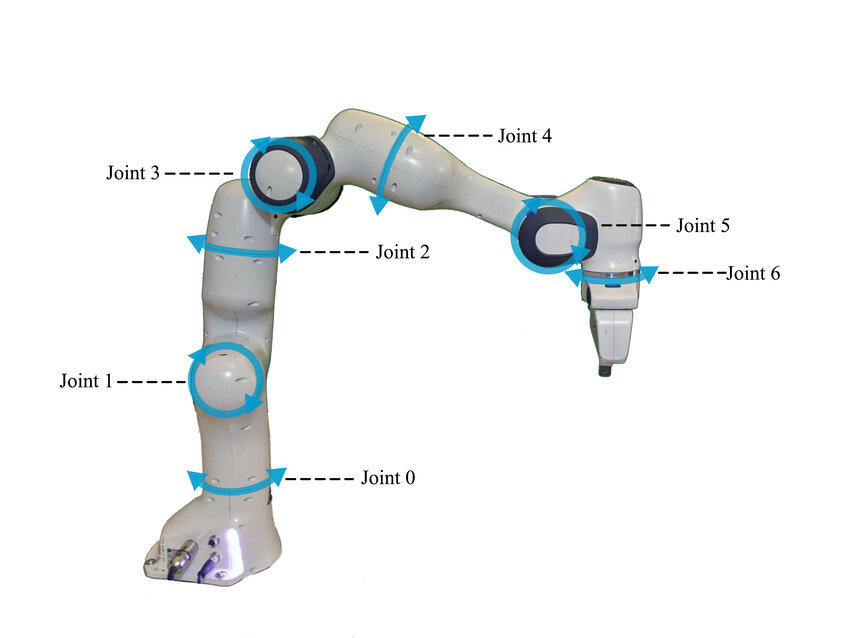
\includegraphics[width=12cm]{img/panda-links-and-joints}
    \caption{Zglobovi i članci na Frank Emika Panda manipulatoru\protect\footnotemark}
    \label{fig:panda-zglob}
\end{figure}
\footnotetext{Preuzeto sa \url{ https://www.researchgate.net/ }}

\subsection{Konfiguracija manipulatora}
Konfiguraciju manipulatora čini potpuno određen položaj svih njegovih točaka.
Skup svih mogućih konfiguracija čini konfiguracijski prostor manipulatora.
Pojedinu konfiguraciju tada možemo promatrati kao točku unutar konfiguracijskog prostora.

Kao i svaki prostor i konfiguracijski prostor ima svoju dimenziju i oblik.
Dimenzija je određena brojem realnih koordinata potrebnih za potpunu reprezentaciju konfiguracije, što još nazivamo i stupnjevi slobode.
Oblik konfiguracijskog prostora je također jako bitan s obzirom da on određuje moguće prepreke i ograničenja unutar samog prostora što smanjuje broj mogućih konfiguracija.
U nastavku ćemo pobliže objasniti što sve utječe na broj stupnjeva slobode manipulatora te kakve sve oblike konfiguracijskog prostora možemo susresti.

\hfill
\subsection{Vrste zglobova i stupnjevi slobode}
Zglobovi i članci zajedno omogućuju da manipulator postigne željena stanja.
Skup svih stanja koje manipulator može dosegnuti u prostoru nazivamo radni prostor robota (eng. \textit{workspace}).
Ono što najviše određuje radni prostor jesu vrste zglobova od kojih se naš manipulator sastoji.

\begin{figure}[H]
    \centering
    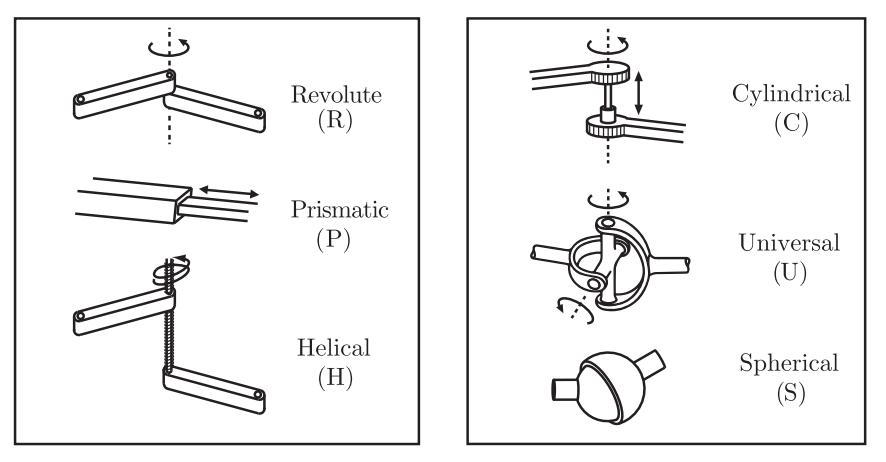
\includegraphics[width=12cm]{img/robot-joints}
    \caption{Vrste zglobova}
    \label{fig:robot-joints}
\end{figure}
\footnotetext{Preuzeto sa \url{ https://hades.mech.northwestern.edu/images/2/25/MR-v2.pdf }}
Na slici \ref{fig:robot-joints} možemo vidjeti različite vrste zglobova koje se koriste.
Svaki od ovih zglobova sastoji se od određenog broja stupnjeva slobode.
Stupnjeve slobode čini broj nezavisnih varijabli koje određuju kretanje nekog tijela.
Kruta tijela u prostoru obično sadrže šest stupnjeva slobode.
Tri stupnja slobode za translaciju, odnosno rotaciju, po svakoj od triju koordinatnih osi.

Kod robotskih manipulatora stupnjeve slbode definiramo na razini zglobova ili manipulatora u cijelosti.
Tako revolucijski zglob sadrži jedan stupanj slobode, odnosno rotaciju oko jedne osi, dok sferični zglob sadrži 3 stupnja slobode te funkcijom podjseća na ljudski rameni zglob.
Ako želimo izraziti broj stupnjeva slobode za manipulator u cijelosti tada se možemo poslužiti Grüblerovom formulom koju možemo vidjeti u formuli (\ref{eq:grubler}).

\begin{equation}
    \begin{aligned}
        \text { dof } &=\underbrace{m(N-1)}_{\text {rigid body freedoms }}-\underbrace{\sum_{i=1}^{J} c_{i}}_{\text {joint constraints }} \\
        &=m(N-1)-\sum_{i=1}^{J}\left(m-f_{i}\right) \\
        &=m(N-1-J)+\sum_{i=1}^{J} f_{i} \cdot
    \end{aligned}
    \label{eq:grubler}
\end{equation}

Varijabla \textit{m} predstavlja konstantu, koja iznosi 3 za planarne manipulatore, odnosno 6 za prostorne manipulatore.
Varijabla \textit{N} predstavlja broj članaka, dok varijabla \textit{J} predstavlja broj zglobova.
Konačno, varijabla \textit{f\textsubscript{i}} predstavlja broj stupnjeva slobode pojedinog zgloba.

\subsection{Oblik konfiguracijskog prostora}
Uz dimenziju konfiguracijskog prostora bitan je i njegov oblik.
Oblik prostora definiran je svojom topologijom, odnosno numeričkom reprezentacijom.

Toplogiju možemo definirati kao skup sličnih oblika prostora, odnosno smatramo da su dva prostora topološki jednaka
ako se jedan prostor može dobiti iz drugog bez "\textit{ljepljenja}" i "\textit{rezanja}"~\cite{10.5555/3165183}.
Tako možemo reći kako su sfera i elipsoid topološki jednaki, dok ravnina i kugla nisu.

Oblik prostora prikazujemo putem njegove numeričke reprezentacije.
Tako točku unutar ravnine predstavljamo s vektorom od dvije dimenzije, dok točku u prostoru predstavljamo s vektorom od tri dimenzije.
Ukoliko je naš prostor sfernog oblika tada točku na sferi možemo prikazati preko dvije veličine kuteva.
Različite numeričke reprezentacije i topologije možemo vidjeti na slici \ref{fig:configuration-topology}

\begin{figure}[H]
    \centering
    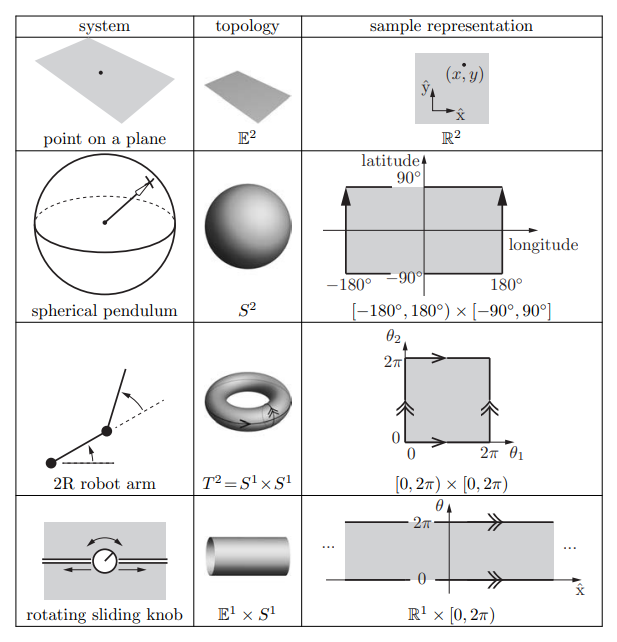
\includegraphics[width=12cm]{img/configuration-topology}
    \caption{Konfiguracijski prostori njihova topologija i numerička reprezentacija}
    \label{fig:configuration-topology}
\end{figure}

\section{Kinematika krutog tijela}
Kruto tijelo ćemo definirati kao idealni sustav točaka koje održavaju iste međusobne razmake~\cite{defKrutogTijela}.
Ranije smo spomenuli kako za potpuno određivanje konfiguracije manipulatora u prostoru moramo znati položaj njegovih točaka.
Da bismo poznavali položaj tih točaka potrebno je definirati u kojem koordinatnog sustavu ih promatramo.
Postoje tri osnovne vrste koordinatnih sustava:
\begin{itemize}
  \item Linijski ili jednodimenzionalni sustavi
  \item Planarni ili dvodimenzionalni sustavi
  \item Prostorni ili trodimenzionalni sustavi
\end{itemize}
\newpage
Zbog toga što u ovom radu promatramo pojmove u konteksu robotskog manipulatora mi ćemo se fokusirati na trodimenzionalni sustav.
Nakon što smo odredili dimenzije našeg koordinatnog sustava potrebno je odrediti koje je njegovo središte.

Koordinatni sustav možemo predstaviti preko prostora unutar kojeg naš mainpulator djeluje što onda nazivamo prostorni oblik (engl. \textit{Space frame}).
Drugi pristup koji možemo koristiti je da predstavimo koordinatni sustav preko neke fiksne točke na našem krutom tijelu što onda nazivamo \textit{tjelesni} oblik (engl. \textit{Body frame}).
U kontekstu našeg manipulatora ta točka bi mogla biti njegova baza ili točka na izvršnom elementu.

U praksi ćemo ipak uvijek htjeti promatrati naš manipulator kroz koordinatni sustav prostora, no onda bismo trebali biti upoznati kako pretvaramo koordinatni sustav našeg manipulatora u prostorni koordinatni sustav.
Za takvu pretvorbu služe nam rotacijske i translacijskse matrice.
Ovo će nam koristiti i u nastavku kod izvoda formule direktne kinematike koju ćemo tada moći jednostavnije i jasnije izvesti.

\subsection{Translacija i rotacija u prostoru}
Translacija je transformacija u prostoru koja svakoj komponenti točke dodaje određeni pomak.
Tako je koordinatni sustav manipulatora translatiran u prostoru u odnosu na prostorni koordinatni sustav.
Matricu translacije u prostornom koordinatnom sustavu u svom općem obliku možemo vidjeti pod (\ref{eq:translacijska-matrica})

\begin{equation}
\boldsymbol{\Psi}_{t r}=\left[
    \begin{array}{cccc}
        1 & 0 & 0 & 0 \\
        0 & 1 & 0 & 0 \\
        0 & 0 & 1 & 0 \\
        \Delta_x & \Delta_y & \Delta_z & 1
    \end{array}
    \right]
    \label{eq:translacijska-matrica}
\end{equation}

Možemo vidjeti kako je ova matrica veličine 4x4, pa možemo postaviti validno pitanje kako ćemo našu trodimenzionalnu točku pomoću ove matrice translatirati u prostoru.
Zato ćemo za računanje s ovakvim oblikom translacijske matrice upotrijebiti homogene koordinate koje ćemo definirati u poopćenom n-dimenzionalnom prostoru~\cite{book:irg}.

\noindent~Ukoliko imamo n-dimenzionalnu točku koja je zadana kao:
\begin{align*}
    \bm T_P=\left(T_{P_1}, T_{P_2}, \ldots, T_{P_n}\right)
\end{align*}
Tada njena homogena reprezentacija ima oblik:
\begin{align*}
    \bm T_{Ph}=\left(T_{Ph_1}, T_{Ph_2}, \ldots, T_{Ph_n}, h\right)
\end{align*}
Gdje definiramo veličinu \textit{h} kao:
\begin{align*}
    \bm T_{P_i}=\frac{T_{P h_i}}{h} \text {, odnosno } T_{P h_i}=T_{P_i} \cdot h \text {. }
\end{align*}
Tako naša 3-dimenzionalna točka postaje 4-dimenzionalna te translaciju dobivamo kao umnožak homogene točke i translacijske matrice:

\begin{equation}
\bold T_{t r}=
\left[
    \begin{array}{cccc}
        x & y & z & 1 \\
    \end{array}
    \right]
\left[
    \begin{array}{cccc}
        1 & 0 & 0 & 0 \\
        0 & 1 & 0 & 0 \\
        0 & 0 & 1 & 0 \\
        \Delta_x & \Delta_y & \Delta_z & 1
    \end{array}
    \right]
    \label{eq:translacijska-matrica-full}
\end{equation}


Inverz ove operacije translacije iz (\ref{eq:translacijska-matrica}) možemo vidjeti pod (\ref{eq:translacijska-matrica-inverz}).
Trivijalno proizlazi da je inverz pomak u negativnom smjeru od onog početnog.
\begin{equation}
    \boldsymbol{\Psi}_{t r}=\left[
        \begin{array}{cccc}
            1 & 0 & 0 & 0 \\
            0 & 1 & 0 & 0 \\
            0 & 0 & 1 & 0 \\
            -\Delta_x & -\Delta_y & -\Delta_z & 1
        \end{array}
        \right]
    \label{eq:translacijska-matrica-inverz}
\end{equation}

\newpage
Rotacija je prostorna transformacija koja točku rotira oko ishodišta za određeni kut $\theta$~\cite{book:irg}.
Pozitivnim smjerom rotacije smatrat ćemo smjer obrnut od kazaljke na satu.
Za rotaciju u prostoru razlikujemo tri moguće rotacije.

Pozitivnu rotaciju oko osi \textit{x}, \textit{y} i \textit{z} u općenitom obliku definiramo pomoću sljedećih rotacijskih matrica:

\begin{equation}
    \boldsymbol{\Psi}_{\text {rotx }}=\left[\begin{array}{cccc}
    1 & 0 & 0 & 0 \\
    0 & \cos (\alpha) & \sin (\alpha) & 0 \\
    0 & -\sin (\alpha) & \cos (\alpha) & 0 \\
    0 & 0 & 0 & 1
    \end{array}\right]
    \label{eq:rotacija-x-matrica}
\end{equation}

\begin{equation}
    \boldsymbol{\Psi}_{\text {roty }}=\left[\begin{array}{cccc}
        \cos (\beta) & 0 & -\sin (\beta) & 0 \\
        0 & 1 & 0 & 0 \\
        \sin (\beta) & 0 & \cos (\beta) & 0 \\
        0 & 0 & 0 & 1
    \end{array}\right]
    \label{eq:rotacija-y-matrica}
\end{equation}

\begin{equation}
    \boldsymbol{\Psi}_{\text {rotz }}=\left[\begin{array}{cccc}
    \cos (\gamma) & \sin (\gamma) & 0 & 0 \\
    -\sin (\gamma) & \cos (\gamma) & 0 & 0 \\
    0 & 0 & 1 & 0 \\
    0 & 0 & 0 & 1
    \end{array}\right]
    \label{eq:rotacija-z-matrica}
\end{equation}
\hfill

Ovakav općeniti oblik rotacijskih i translacijskih matrica nam nije previše pogodan za računanje.
Htjeli bismo pomoću jedne matrice odrediti položaj i orjentaciju manipulatora u prostornom koordinatnom sustavu.
Zbog toga uvodimo homogene tranformacijske matrice
\newpage
\subsection{Homogene transformacijske matrice}
Homogene transformacijske matrice definirat ćemo preko Euklidske \textit{SE(3)} grupe.
Euklidsku grupu čine sve transformacije, poput rotacije ili translacije, koje čuvaju udaljenost između točaka u prostoru.
Našu \textit{SE(3)} grupu definirat ćemo kao sve 4 x 4 realne matrice sljedećeg oblika~\cite{10.5555/3165183}:

\begin{equation}
    T=\left[\begin{array}{cc}
    R & p \\
    0 & 1
    \end{array}\right]=\left[\begin{array}{cccc}
    r_{11} & r_{12} & r_{13} & p_1 \\
    r_{21} & r_{22} & r_{23} & p_2 \\
    r_{31} & r_{32} & r_{33} & p_3 \\
    0 & 0 & 0 & 1
    \end{array}\right]
    \label{eq:transformacijska matrica}
\end{equation}

Ove matrice imaju i neka zanimljiva svojstva.
Jedno od njih je da je inverz transformacijske matrice također transformacijska matrica te ima oblik definiran u (\ref{eq:inverz-transformacijske}).
Ovo svojstvo nam može biti korisno kada želimo neku točku prikazati unutar koordinatnog sustava manipulatora a znamo njenu prostornu reprezentaciju.
\begin{equation}
    T^{-1}=\left[\begin{array}{cc}
    R & p \\
    0 & 1
    \end{array}\right]^{-1}=\left[\begin{array}{cc}
    R^{\mathrm{T}} & -R^{\mathrm{T}} p \\
    0 & 1
    \end{array}\right]
\label{eq:inverz-transformacijske}
\end{equation}

Drugo svojstvo je da je umnožak dvije transformacijske matrice također transformacijska matrica.
Ovo svojstvo će nam biti korisno kod izračuna direktne kinematike.
Množenje transformacijskih matrica je također asocijativna operacija, ali nije komutativna.
Zbog svih svojih svojstava homogene transformacijske matrice koriste se za:
\begin{itemize}
    \item Reprezentaciju položaja i orjentacije krutog tijela u prostoru
    \item Transformaciju točke ili vektora iz jednog koordinatnog sustava u drugi
    \item Pomicanje vektora ili koordinatnog sustava
\end{itemize}

\newpage
\section{Direktna kinematika}
Direktna kinematika služi za izračun položaja i orjentacije izvršnog elementa uz poznati iznos kutova pojedinog zgloba manipulatora.
Veoma je bitna zbog toga što upravo tim izračunom možemo saznati konfiguraciju izvršnog elementa manipulatora kako bismo izvršili neku nama korisnu radnju.
Direktnu kinematiku možemo računati u koordinatnom sustavu robota ili u prostornom koordinatnom sustavu.
Mi ćemo se u nastavku fokusirati samo na prostorni oblik pošto nam je on korisniji kod upravljanja manipulatorom u stvarnom svijetu, pogotovo ako su pristune neke prepreke unutar prostora.

U formuli direktne kinematike koristit ćemo transformacijske matrice za transformaciju položaja i orjentacije između koordinatnih sustava svakog pojedinog zgloba.
Tako ćemo kod Panda robota, kojeg smo promatrali, za izračun direktne kinematike imati sedam transformacijskih matrica za susjedne zglobove.
Formula za izračun direktne kinematike tada će biti definirana u formuli (\ref{eq:equation-direktna-kinematika}):
\begin{equation}
T_{07}=T_{01} T_{12} T_{23} T_{34} T_{45} T_{56} T_{67}
    \label{eq:equation-direktna-kinematika}
\end{equation}

Sada nam preostaje odrediti pojedinačne transformacijske matrice za susjedne zglobove.
Ovo možemo odrediti pomoću dva pristupa.
Prvi pristup koristi PoE formulu, dok se drugi pristup oslanja na DH (Denavit-Hartenberg) parametre.
\subsection{PoE formula}
Prvi pristup koristi takozvanu PoE (engl. \textit{Product of exponentials formula}) formulu.
Za izračun putem ovog pristupa potrebne su nam sljedeće varijable:
\begin{itemize}
    \item Matrica \textit{M} koja predstavlja položaj i orjentaciju izvršnog elementa kada je manipulator u početnom stanju, odnosno kada su svi kutovi zglobova jednaki 0
    \item Matrice \textit{$S_1, ..., S_7$} koje odgovaraju translaciji i rotaciji u odnosu na središte prostornog koordinatnog sustava kada je manipulator u početnom stanju te rotira oko zgloba
    \item Konfiguracija kuteva \textit{$\theta_1, ..., \theta_7$} koje predstavljaju zaokret pojedinog zgloba
\end{itemize}
\newpage
Radi lakšeg računanja matrica \textit{M} te sve matrice \textit{S} zapisane su u svom \textit{SE(3)} obliku.
Tako matrica S inicijalno izgleda kao stupac vektor što možemo vidjeti u (\ref{eq:s-matrica-stupac}).
Prve 3 veličine predstavljaju translaciju u prostornom koordinatnom sustavu, dok zadnje 3 veličine predstavljaju rotaciju.

\begin{equation}
    \mathcal{S}_i=\left[\begin{array}{c}
    \omega \\
    v
    \end{array}\right]=\left[\begin{array}{c}
    \omega_1 \\
    \omega_2 \\
    \omega_3 \\
    v_1 \\
    v_2 \\
    v_3
    \end{array}\right]
    \label{eq:s-matrica-stupac}
\end{equation}

Želimo li matricu \textit{$S_i$} izraziti preko standardne \textit{SE(3)} reprezentacije tada dobivamo matricu u (\ref{eq:s-matrica-se3})

\begin{equation}
    \left[S_3\right]=\left[\begin{array}{cc}
    [\omega] & v \\
    0 & 0
\end{array}\right]=
    \left[\begin{array}{cccc}
        w_{11} & w_{12} & w_{13} & v_1 \\
        w_{21} & w_{22} & w_{23} & v_2 \\
        w_{31} & w_{32} & w_{33} & v_3 \\
        0 & 0 & 0 & 1
    \end{array}\right]
    \label{eq:s-matrica-se3}
\end{equation}

Koristeći matrice \textit{$S_i$} i matricu \textit{M} zamjenjujemo homogene transformacijske matrice njihovom eksponencijalnom reprezentacijom.
Tako će homogena transformacijska matrica za zglob \textit{i} biti definirana preko svoje eksponencijalne reprezentacije koju možemo vidjeti u (\ref{eq:eksponencijalna-reprezentacija})

\begin{equation}
     T_{0i}=e^{\left[\mathcal{S}_{1}\right] \theta_{1}}  e^{\left[\mathcal{S}_{2}\right] \theta_{2}} , ..., e^{\left[\mathcal{S}_{i-1}\right] \theta_{i-1}} e^{\left[\mathcal{S}_{i}\right] \theta_{i}} M
    \label{eq:eksponencijalna-reprezentacija}
\end{equation}

\subsection{DH parametri}

%-------------------------------------------------------------------------------
\chapter{Rezultati i rasprava}
\label{pog:rezultati_i_rasprava}



%--- ZAKLJUČAK / CONCLUSION ----------------------------------------------------
\chapter{Zaključak}
\label{pog:zakljucak}



%--- LITERATURA / REFERENCES ---------------------------------------------------

% Literatura se automatski generira iz zadane .bib datoteke / References are automatically generated from the supplied .bib file
% Upiši ime BibTeX datoteke bez .bib nastavka / Enter the name of the BibTeX file without .bib extension
\bibliography{literatura}



%--- SAŽETAK / ABSTRACT --------------------------------------------------------

% Sažetak na hrvatskom
\begin{sazetak}
  Unesite sažetak na hrvatskom.

  \blindtext
\end{sazetak}

\begin{kljucnerijeci}
  prva ključna riječ; druga ključna riječ; treća ključna riječ
\end{kljucnerijeci}


% Abstract in English
\begin{abstract}
  Enter the abstract in English.
  
  \blindtext 
\end{abstract}

\begin{keywords}
  the first keyword; the second keyword; the third keyword
\end{keywords}


%--- PRIVITCI / APPENDIX -------------------------------------------------------

% Sva poglavlja koja slijede će biti označena slovom i riječi privitak / All following chapters will be denoted with an appendix and a letter
\backmatter


\Blindtext


\end{document}
